\documentclass[a4paper,12pt,notitlepage,openany]{article}
\usepackage{url}
%\usepackage[dvips]{graphicx}
%\usepackage{graphics}
\usepackage[spanish]{babel}
%\selectlanguage{spanish}
%\usepackage[T1]{fontenc}
\usepackage[latin1]{inputenc}
\usepackage{babel}
%\usepackage{named}
\usepackage{geometry}
\usepackage{makeidx}
\usepackage{graphicx}

% Espaciado por defecto, (no afecta a figuras, minipages, pie de pagina...)
\usepackage{setspace}
%\setstretch{1.35}
%\setstretch{1.2}

%para subfiguras
\usepackage[normalsize]{subfigure}
\renewcommand{\subfigtopskip}{0pt}
\renewcommand{\subfigcapskip}{0pt}
\renewcommand{\subfigbottomskip}{0pt}

% Definimos el margen y el tipo de letra de los pies de figura
\usepackage[normal,bf]{caption2}
\setlength{\captionmargin}{20pt}
\renewcommand{\captionfont}{\footnotesize\slshape}
%\newcommand{\mycaption}[1]{\caption{\textit{\small{#1}}}} 

%Para que la bibliografia salga en el indice:
\let\OLDthebibliography=\thebibliography
\def\thebibliography#1{\OLDthebibliography{#1}%
  \addcontentsline{toc}{section}{\bibname}}

%\geometry{left=3cm, right=3cm, top=3cm, bottom=3cm}
%\geometry{inner=2.5cm, outer=1.5cm, top=2cm, bottom=2cm}

\makeindex

\selectlanguage{spanish}
\bibliographystyle{plain}

\title{Manual de la biblioteca Progeo}
\author{Manuel Mendoza}
\date{Universidad Rey Juan Carlos}

\begin{document}
\maketitle
\tableofcontents

\section{Introducci\'on}

La biblioteca \textit{Progeo} se ha incorporado recientemente a la plataforma \textit{jdec}. Esta librer\'{i}a nos ayuda con la geometr\'{i}a proyectiva cuando tratamos con c\'{a}maras. Basandose en los parametros intr\'{i}nsecos (centro de la imagen, distancia focal...) y los parametros extr\'{i}nsecos (posici\'{o}n de la c\'{a}mara, hacia d\'{o}nde mira, con qu\'{e} roll...) es capaz de calcular donde se proyectar\'{i}a un punto (x,y,z) en 3D en nuestra c\'{a}mara, y viceversa.

\section{Importando c\'{a}maras de ARToolKit}

\textit{ARToolKit} \footnote{\label{1}http://www.hitl.washington.edu/artoolkit/download/} es una herramienta de calibraci\'{o}n desarrollada en conjunto por las universidades de Osaka, Washington y Canterbury. Mediante una serie de patrones diferentes nos ayuda a obtener los parametros intr\'{i}nsecos y extr\'{i}nsecos de la c\'{a}mara. Con los programas de calibraci\'{o}n (\textit{calib\_dist} y \textit{calib\_cparam}) obtenemos el centro de la imagen, la distorsi\'{o}n por el tama\~{n}o de los p\'{i}xeles y la distancia focal. Con \textit{exview} obtenemos los parametros extr\'{i}nsecos, un vector 3D con la posici\'{o}n de la c\'{a}mara y un \textit{quaternion} que nos indica hacia d\'{o}nde mira la c\'{a}mara y el roll con el que lo hace.

A continuaci\'{o}n vamos a ver la estructura de una c\'{a}mara en progeo.
\begin{verbatim}
typedef struct {
  HPoint3D position; /* camera 3d position in mm */
  HPoint3D foa; /* camera 3d focus of attention in mm */
  float roll; /* camera roll position angle in rads */
  float fdist; /* focus distance in mm*/
  float u0,v0; /* pixels */
  /* camera K matrix */
  float k11,k12,k13,k14,k21,k22,k23,k24,k31,k32,k33,k34;
  /* camera rotation + translation matrix */
  float rt11,rt12,rt13,rt14,rt21,rt22,rt23,rt24,rt31,rt32...;
  /* top right and bottom left points */
  HPoint3D tr, bl;
  /* name */
  char name[256];
}TPinHoleCamera;
\end{verbatim}

Esta estructura la "rellenamos" con los datos que nos da \textit{ARToolKit}. Con los programas de calibraci\'{o}n obtendremos la distancia focal (\textit{fdist}) y el centro de la imagen (\textit{u0,v0}), y los dem\'{a}s datos que forman parte de la matriz K (\textit{k11,k12,k13,k14,k21,k22...}):

\[
K = \left( \begin{array}{lcr}
            f_h     & s   		& u_0  \\
            0     	& f_v   	& v_0  \\
            0				& 0				& 1
           \end{array}
    \right)
\]

\begin{figure}[htb]
	\begin{center}
		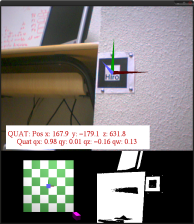
\includegraphics{figs/exview2}
	\end{center}
	\caption[Figura 1]{Ejecuci\'{o}n normal de \textit{exview}}
\end{figure}

 Con \textit{exview} obtendremos la posicion de la c\'{a}mara (\textit{position}) y el resto de par\'{a}metros de la matriz de rotaci\'{o}n+traslaci\'{o}n(\textit{rt11,rt12,rt13,rt14,rt21,rt22...}) los obtendremos a partir del quaterni\'{o}n mediante las siguientes ecuaciones:

\[
RT = \left( \begin{array}{l}
							\underline{R \quad | -RC} \\
							0 \quad 0 \quad 0 \quad 1
							\end{array}
			\right)
\]

$ rt_{11}= q_w^2 + q_x^2 - q_y^2 - q_z^2 $\\
$ rt_{12}= 2 * (q_x*q_y - q_w*q_z)$\\
$ rt_{13}= 2 * (q_w*q_y + q_x*q_z)$\\
$ rt_{14}= -x * rt_{11} - y * rt_{12} - z * rt_{13}$\\
$ rt_{21}= 2 * (q_x*q_y + q_w*q_z)$\\
$ rt_{22}= q_w^2 - q_x^2 + q_y^2 - q_z^2$\\
$ rt_{23}= 2 * (q_y*q_z - q_w*q_x)$\\
$ rt_{24}= -x * rt_{21} - y * rt_{22} - z * rt_{23}$\\
$ rt_{31}= 2 * (q_x*q_z - q_w*q_y)$\\
$ rt_{32}= 2 * (q_w*q_x + q_y*q_z)$\\
$ rt_{33}= q_w^2 - q_x^2 - q_y^2 + q_z^2$\\
$ rt_{34}= -x * rt_{31} - y * rt_{32} - z * rt_{33}$\\
$ rt_{41}= 0$\\
$ rt_{42}= 0$\\
$ rt_{43}= 0$\\
$ rt_{44}= 1$\\


S\'{o}lo resta una observaci\'{o}n, y es que en \textit{ARToolKit} se trabaja con imagenes en un tama\~{n}o de 640x480 y en \textit{jde} se trabaja con imagenes en 320x240 por lo que tendremos que dividir a la mitad tanto el centro de la imagen como la distancia focal.


\nocite{*}
%\bibliographystyle{alpha}
\end{document}
